% Progress report for Oliver and Dr. Soleimani, October 2026 (same content as slides_progress_2026-10.pptx,
% in the format of slides_1005 / slides_coupling_1020).
% Build: pdflatex slides_progress_1024.tex (twice). Rules: CLAUDE.md "Slides, notes and other documents".
% The two videos are linked with \movie (play in Acrobat/Okular; the PDF shows the last frame otherwise);
% keep assets/anim_coupled_tvd_*_ab_inherit.mp4 next to the PDF when sending it.
\documentclass[aspectratio=169,11pt]{beamer}
\usetheme{default}
\usefonttheme{serif}
\usefonttheme{professionalfonts}
\usepackage[T1]{fontenc}
\usepackage{mathptmx}           % Times text and mathematics, as the thesis figures
\usepackage{booktabs}
\usepackage{array}
\usepackage{amsmath,amssymb}
\usepackage{xcolor}
\usepackage{graphicx}
\usepackage{caption}
\captionsetup{font=scriptsize,labelfont=bf,skip=2pt}
\usepackage{multimedia}
\usepackage{pgfplots}
\pgfplotsset{compat=1.17}

\definecolor{c3}{RGB}{20,50,100}
\definecolor{warn}{RGB}{180,40,40}
\definecolor{tvd}{RGB}{46,125,107}
\definecolor{lw}{RGB}{217,149,42}
\definecolor{ad}{RGB}{127,140,141}
\setbeamercolor{frametitle}{fg=c3}
\setbeamercolor{structure}{fg=c3}
\setbeamercolor{block title}{fg=c3,bg=c3!8}
\setbeamercolor{block body}{bg=gray!5}
\setbeamerfont{frametitle}{size=\large,series=\bfseries}
\setbeamertemplate{frametitle}{\vspace{4pt}\insertframetitle\par\vspace{-2pt}{\color{c3}\rule{\linewidth}{0.6pt}}}
\setbeamertemplate{navigation symbols}{}
\setbeamertemplate{itemize items}{\textbullet}
\setbeamertemplate{enumerate items}[default]
\setbeamertemplate{caption}[numbered]
\setbeamertemplate{blocks}[default]
\setbeamertemplate{footline}{\hspace{1em}{\tiny\color{gray}K. Nishioka, Coupling the point model to the growth field,
  October 2026}\hfill{\tiny\color{gray}\insertframenumber}\hspace{1em}\vspace{4pt}}
\setbeamertemplate{title page}{\centering\vspace{1.2cm}
  {\color{c3}\LARGE\bfseries\inserttitle\par}\vspace{4pt}{\large\insertsubtitle\par}\vspace{0.8cm}
  {\insertauthor\par}\vspace{2pt}{\small\insertinstitute\par}\vspace{6pt}{\small\insertdate\par}}

\title{Coupling the Point Model to the Growth Field}
\subtitle{Progress since the meeting of 20 October 2026}
\author[Keisuke Nishioka]{Keisuke Nishioka}
\institute[IKM, LUH]{Institute of Continuum Mechanics (IKM), Leibniz Universit\"at Hannover}
\date{October 2026}

\begin{document}
\maketitle

% --------------------------------------------------------
\begin{frame}{Where the coupling stands}
\begin{itemize}\setlength{\itemsep}{8pt}
  \item Implemented as agreed in your element: the point model (Klempt et al.\ 2026) runs at every Gauss point as
        published, consumption by the living biomass $\sum_i\bar\phi_i$, antibiotic in the second nutrient field.
        A Python version solves the same equations.
  \item Composition is robust: $\sum_i\bar\phi_i$, the shares and $c$ agree between the two codes and change by
        less than 1\,\% from $16^3$ to $128^3$.
  \item The front term of Eq.\ 34 needs care: at the paper's $r$ the cell P\'eclet number is about
        \textbf{31} on $16^3$, so a central gradient oscillates.
  \item With a second-order scheme the seed von Mises stress converges to \textbf{$6.2\times10^{-4}$\,Pa}
        (separate example, from $32^3$ on).
\end{itemize}
\end{frame}

% --------------------------------------------------------
\begin{frame}{The coupling agreed on 20 October}
\centering
\begin{figure}
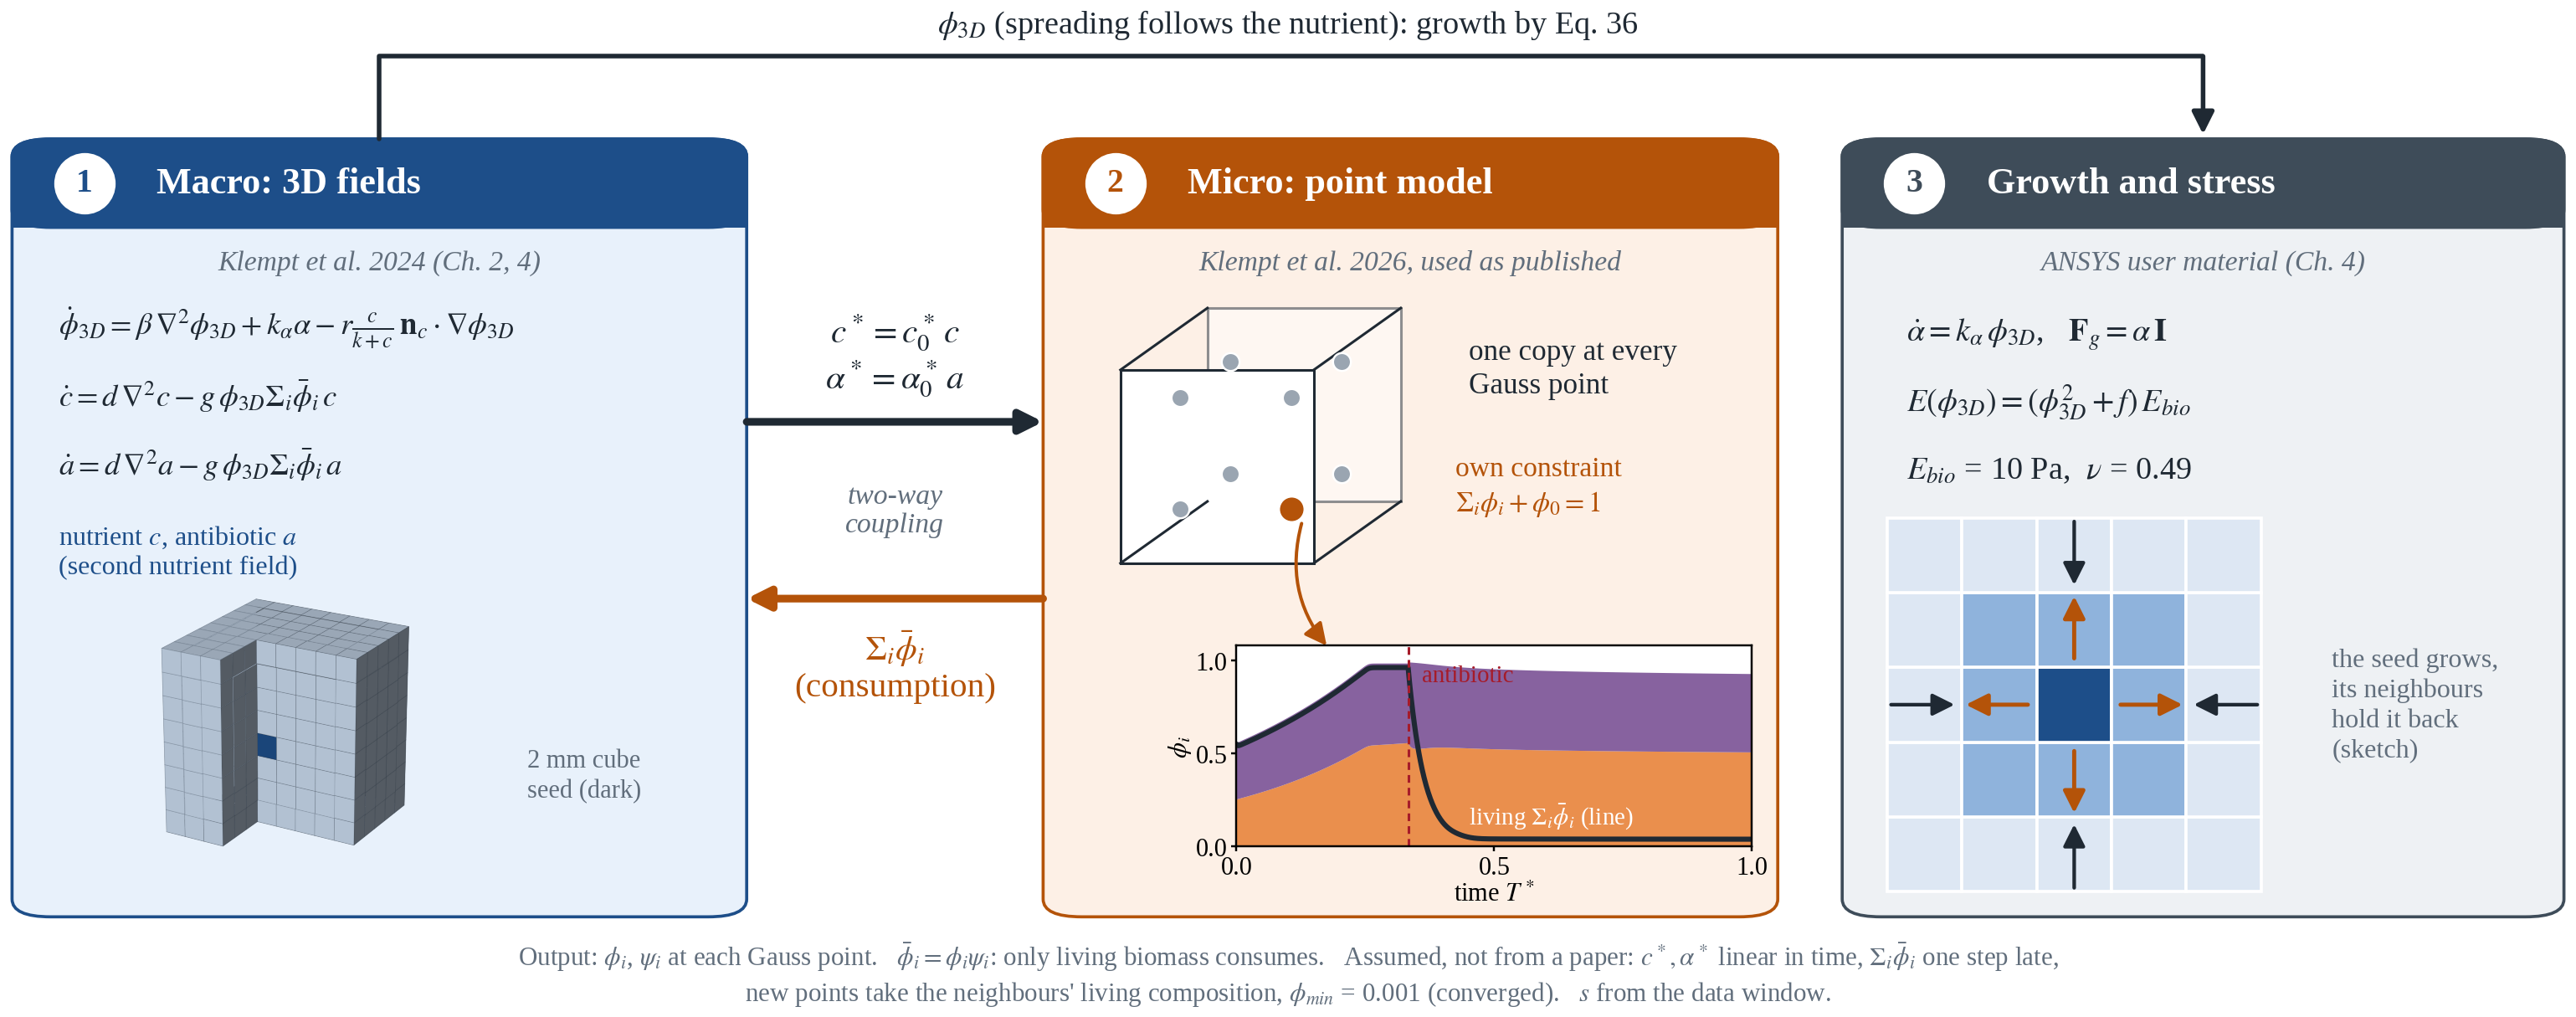
\includegraphics[width=\linewidth,height=0.68\textheight,keepaspectratio]{assets/fig_coupling_schematic_agreed.png}
\caption{Agreed coupling: the 3D fields of Klempt et al.\ (2024) pass $c^*$ and $\alpha^*$ to the point model of
Klempt et al.\ (2026) at each Gauss point, which returns $\sum_i\bar\phi_i$ for the consumption in Eq.\ 35.}
\end{figure}
\end{frame}

% --------------------------------------------------------
\begin{frame}{Separate example with antibiotic}
\centering
\movie[width=0.72\linewidth,height=0.279\linewidth,poster,showcontrols,externalviewer]{%
  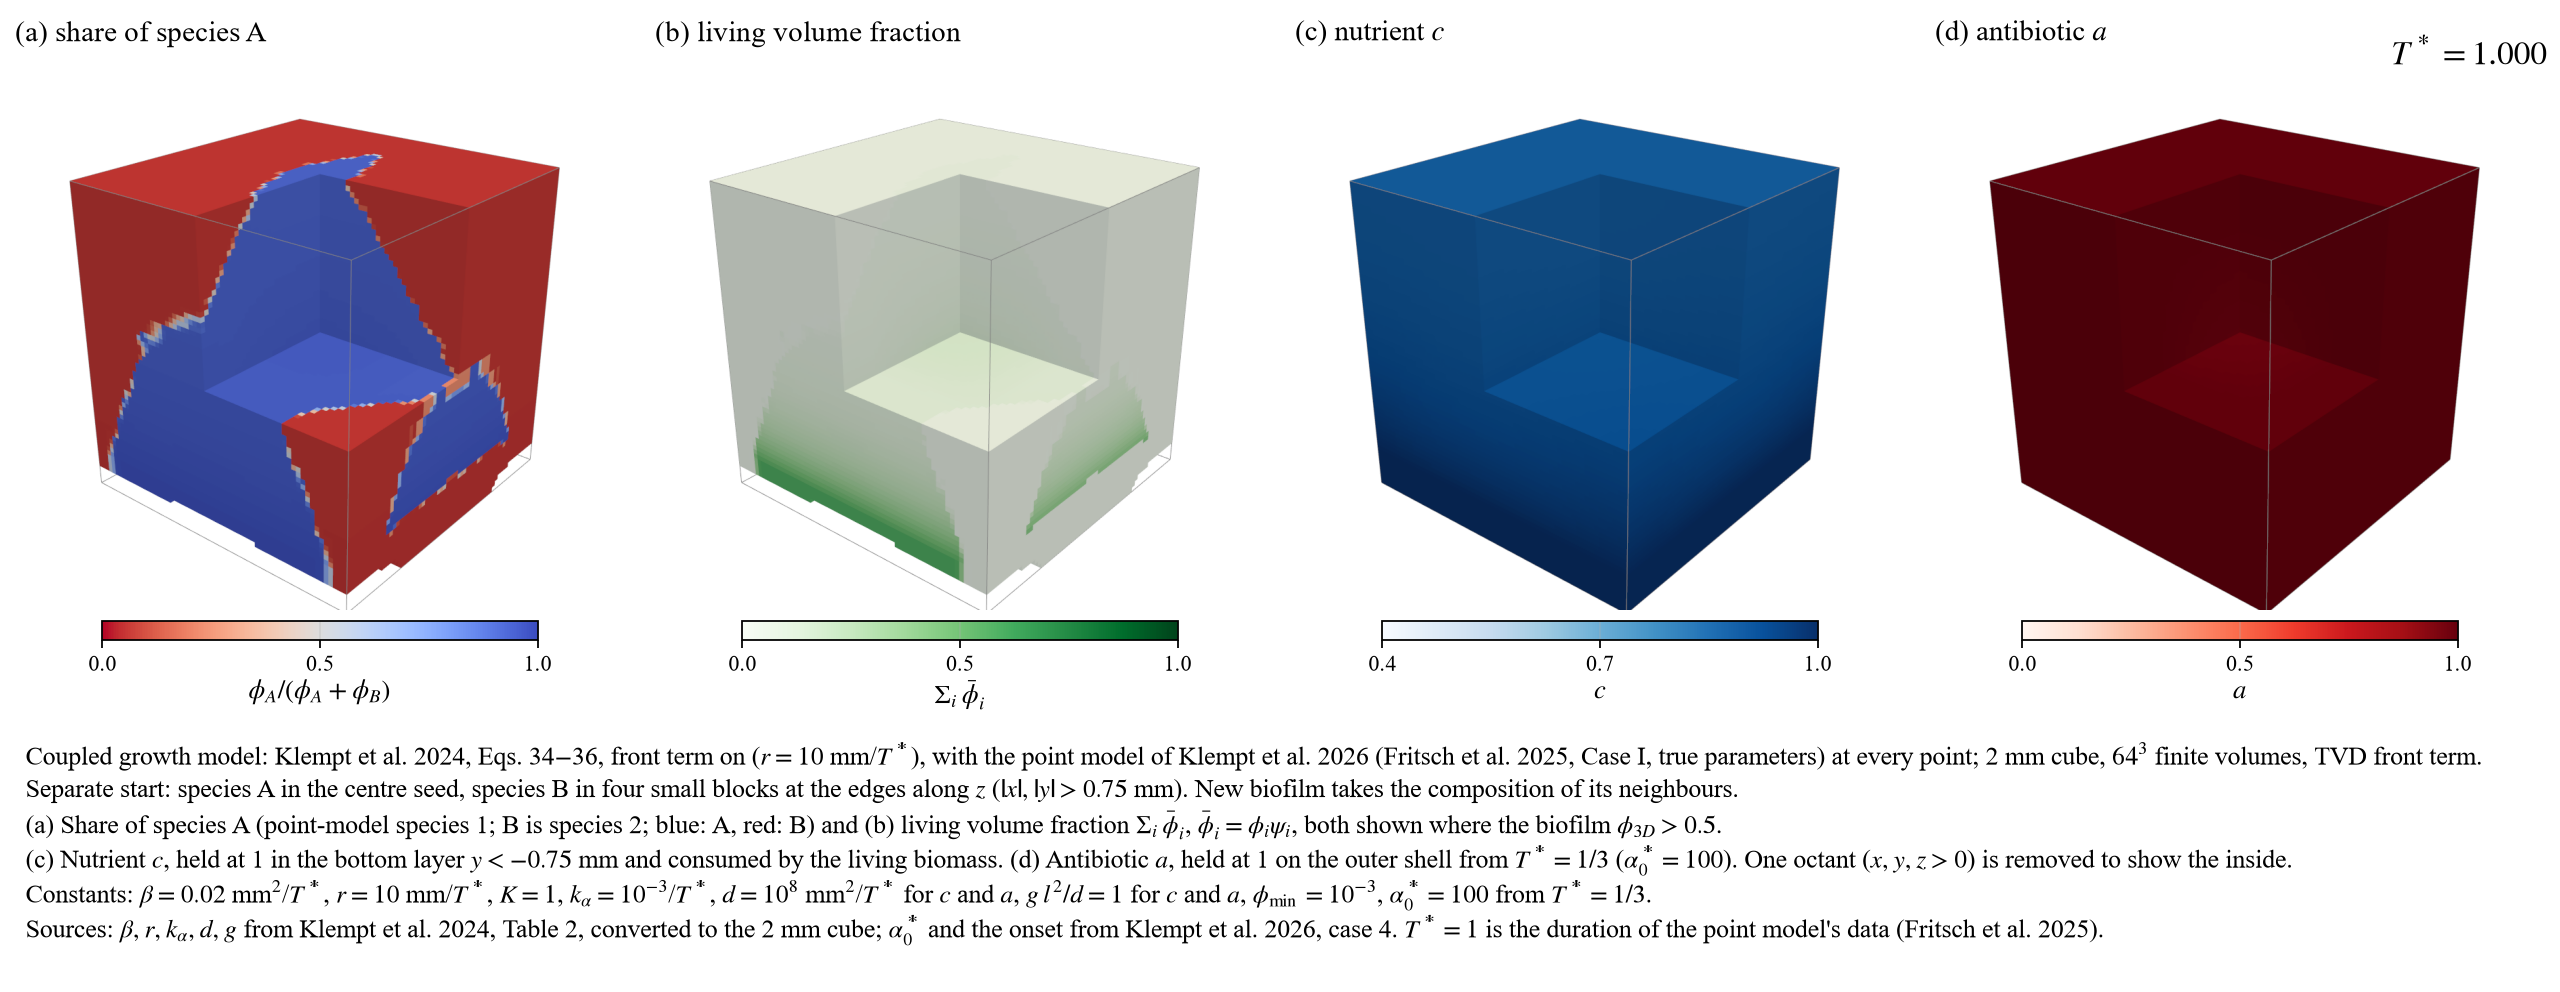
\includegraphics[width=0.72\linewidth]{assets/anim_coupled_tvd_separate_ab_inherit_end.png}}%
  {assets/anim_coupled_tvd_separate_ab_inherit.mp4}
\captionof{figure}{Separate start, $T^*=1$: (a) $\phi_1/(\phi_1+\phi_2)$, (b) $\sum_i\bar\phi_i$, (c) $c$, (d) $a$.
Python, $64^3$.}
\begin{itemize}\small
  \item A (point-model species 1) in the seed, B (species 2) in four blocks at the $z$ edges; nutrient from the
        bottom, antibiotic from all outer faces from $T^*=1/3$ ($\alpha^*_0=100$)
  \item Newly reached cells take the composition of the biofilm they grow from; the antibiotic kills B and,
        where the nutrient is low, A
\end{itemize}
\end{frame}

% --------------------------------------------------------
\begin{frame}{Mixed example with antibiotic}
\centering
\movie[width=0.72\linewidth,height=0.279\linewidth,poster,showcontrols,externalviewer]{%
  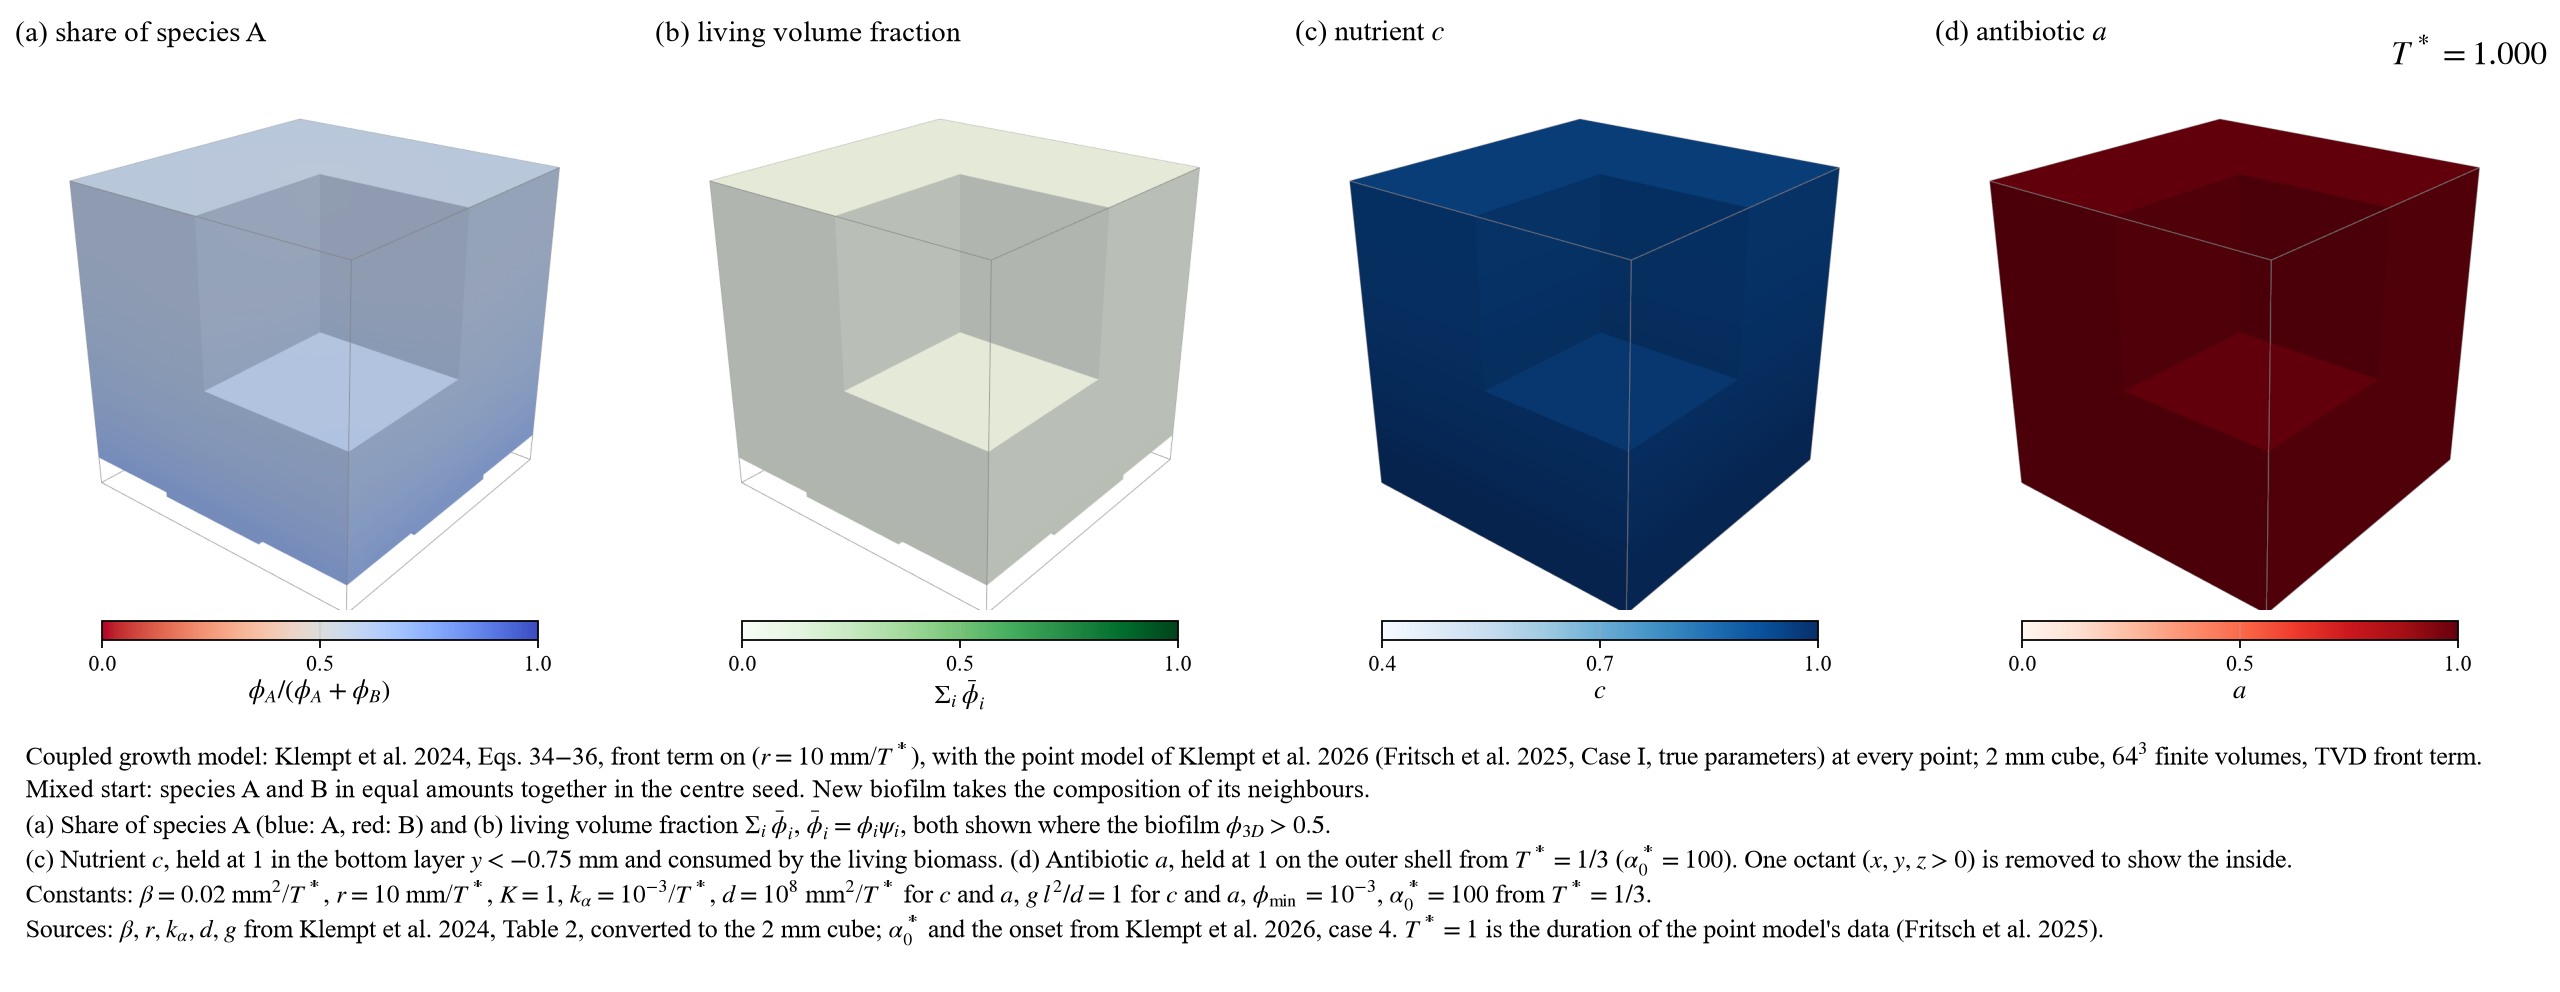
\includegraphics[width=0.72\linewidth]{assets/anim_coupled_tvd_mixed_ab_inherit_end.png}}%
  {assets/anim_coupled_tvd_mixed_ab_inherit.mp4}
\captionof{figure}{Mixed start, $T^*=1$: (a) $\phi_1/(\phi_1+\phi_2)$, (b) $\sum_i\bar\phi_i$, (c) $c$, (d) $a$.
Python, $64^3$.}
\begin{itemize}\small
  \item A and B start together in the seed with equal amounts; same nutrient and antibiotic as before
  \item The antibiotic acts where $c^*=c^*_0c$ falls below $\alpha^* b_i$: the nutrient field decides where it kills
\end{itemize}
\end{frame}

% --------------------------------------------------------
\begin{frame}{Five examples on the finest grid}
\centering\small
\captionof{table}{Seed means at $T^*=1$ (Python, $128^3$, TVD front term).}
\begin{tabular}{lccccc}
\toprule
Example & $\sum_i\bar\phi_i$ & $\phi_1/(\phi_1+\phi_2)$ & $c$ & $\alpha-1$ & von Mises [Pa]\\
\midrule
Separate                          & 0.965 & 0.978 & 0.539 & $9.32\times10^{-4}$ & $6.18\times10^{-4}$\\
Separate, antibiotic              & 0.147 & 0.951 & 0.910 & $9.33\times10^{-4}$ & $6.05\times10^{-4}$\\
Mixed, equal amounts              & 0.960 & 0.848 & 0.578 & $9.07\times10^{-4}$ & $4.87\times10^{-4}$\\
Mixed, equal amounts, antibiotic  & 0.038 & 0.613 & 0.970 & $9.05\times10^{-4}$ & $4.26\times10^{-4}$\\
Mixed (0.25, 0.30), antibiotic    & 0.037 & 0.511 & 0.971 & $9.04\times10^{-4}$ & $4.29\times10^{-4}$\\
\bottomrule
\end{tabular}

\vspace{2pt}{\scriptsize Constants: Klempt et al.\ (2024), Table 2, converted; Fritsch et al.\ (2025), case I;
$\alpha^*_0=100$ from $T^*=1/3$ (Klempt et al.\ 2026, case 4).}
\begin{itemize}\small
  \item The antibiotic lowers the living fraction of the seed from 0.965 to 0.147 (separate) and from 0.960 to
        0.038 (mixed)
  \item $\alpha-1$ hardly changes between examples (Eq.\ 36 is unchanged): the composition reaches the stress
        through $c$ and the front term
\end{itemize}
\end{frame}

% --------------------------------------------------------
\begin{frame}{The front term is an advection}
\begin{columns}[T]
\column{0.38\textwidth}
\[\mathrm{Pe}=\frac{r\,h}{2\beta}\approx 31\]
on $16^3$ ($r=10$\,mm/$T^*$, $\beta=0.02$\,mm$^2$/$T^*$). With a central gradient $\phi_{3D}$ oscillates and the
element stops after two increments; a smaller time step does not help.
\column{0.6\textwidth}\small
\begin{block}{Constant added diffusion $r h/4$}
First order. Stable in the element, but the stress on $16^3$ is about a quarter of the converged value.
\end{block}
\begin{block}{Lax--Wendroff term with an extremum sensor}
Used in the element: second order away from extrema, $\phi_{3D}$ stays in $[0,1]$; on $16^3$ it matches Python with
the same form.
\end{block}
\begin{block}{TVD upwinding (MUSCL, minmod)}
Used in Python for the main results; converged from $64^3$ on.
\end{block}
\end{columns}
\end{frame}

% --------------------------------------------------------
\begin{frame}{Growth converges for every scheme, stress only for second-order ones}
\centering
\pgfplotsset{every axis/.style={width=0.49\linewidth,height=0.52\textheight,xmode=log,log basis x=2,
  xtick={16,24,32,48,64,128},xticklabels={$16^3$,$24^3$,$32^3$,$48^3$,$64^3$,$128^3$},
  tick label style={font=\scriptsize},label style={font=\small},title style={font=\small},grid=major,
  grid style={gray!25},mark size=1.8pt}}
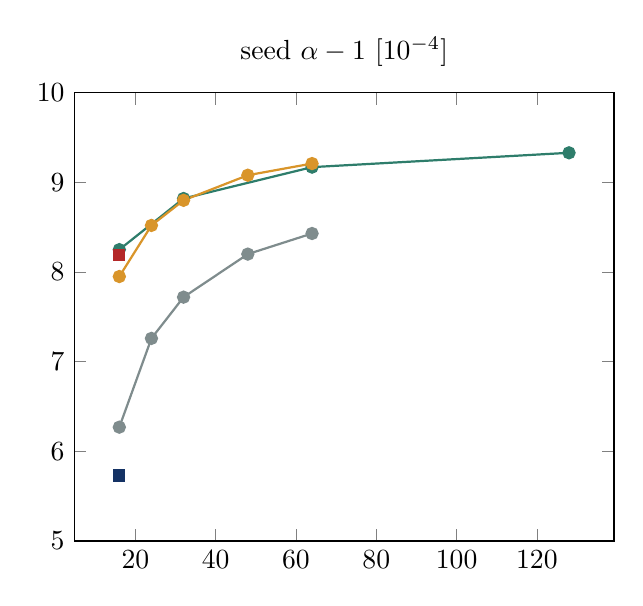
\begin{tikzpicture}
\begin{axis}[title={seed $\alpha-1$ [$10^{-4}$]},ymin=5,ymax=10]
\addplot[tvd,thick,mark=*] coordinates {(16,8.25)(32,8.82)(64,9.17)(128,9.33)};
\addplot[lw,thick,mark=*] coordinates {(16,7.95)(24,8.52)(32,8.80)(48,9.08)(64,9.21)};
\addplot[ad,thick,mark=*] coordinates {(16,6.27)(24,7.26)(32,7.72)(48,8.20)(64,8.43)};
\addplot[warn,only marks,mark=square*] coordinates {(16,8.19)};
\addplot[c3,only marks,mark=square*] coordinates {(16,5.73)};
\end{axis}
\end{tikzpicture}\hfill
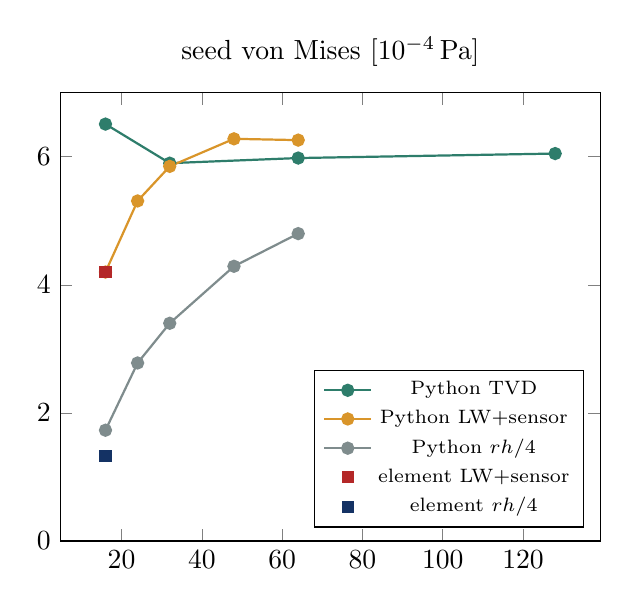
\begin{tikzpicture}
\begin{axis}[title={seed von Mises [$10^{-4}$\,Pa]},ymin=0,ymax=7,legend pos=south east,
  legend style={font=\scriptsize}]
\addplot[tvd,thick,mark=*] coordinates {(16,6.51)(32,5.90)(64,5.98)(128,6.05)};
\addplot[lw,thick,mark=*] coordinates {(16,4.20)(24,5.31)(32,5.85)(48,6.28)(64,6.26)};
\addplot[ad,thick,mark=*] coordinates {(16,1.73)(24,2.78)(32,3.40)(48,4.29)(64,4.80)};
\addplot[warn,only marks,mark=square*] coordinates {(16,4.20)};
\addplot[c3,only marks,mark=square*] coordinates {(16,1.33)};
\legend{Python TVD,Python LW+sensor,Python $rh/4$,element LW+sensor,element $rh/4$}
\end{axis}
\end{tikzpicture}

\captionof{figure}{Seed means of the separate example with antibiotic at $T^*=1$ against the grid ($h=2$\,mm$/n$).
Element: your element with the agreed coupling (ANSYS), $16^3$ so far.}
\end{frame}

% --------------------------------------------------------
\begin{frame}{What the comparison found in the element and in Python}
\small
\begin{columns}[T]
\column{0.49\textwidth}
\begin{block}{Surface points of the element}
$\phi$ at the surface points was an inverse-distance mean that also took inner points; at a wall with
$\phi=1$ it came out low and $\phi$ leaked through the wall. Taking the nearest Gauss point reduced the leak to a
quarter.
\end{block}
\begin{block}{Neighbour selection}
The search keeps the first 30 points in element order; on $16^3$ and $24^3$ the stencils became asymmetric inside
the domain. Selecting by distance makes them symmetric to $10^{-15}$.
\end{block}
\column{0.49\textwidth}
\begin{block}{Column sums of the NEM Laplacian}
The rows sum to zero, the columns do not, so the operator does not conserve $\phi$ with equal weights. A
conservative form removes the rest of the leak.
\end{block}
\begin{block}{Python wall gradient}
My Python version took a one-sided gradient in the wall cells for the front term; corrected to the zero-flux mirror.
After both corrections the codes agree on $8^3$ within 1 to 5\,\%.
\end{block}
\end{columns}
\end{frame}

% --------------------------------------------------------
\begin{frame}{Growth around rigid bars (Klempt 2024, Sect.\ 4.3)}
\begin{columns}[T]
\column{0.64\textwidth}
\begin{figure}
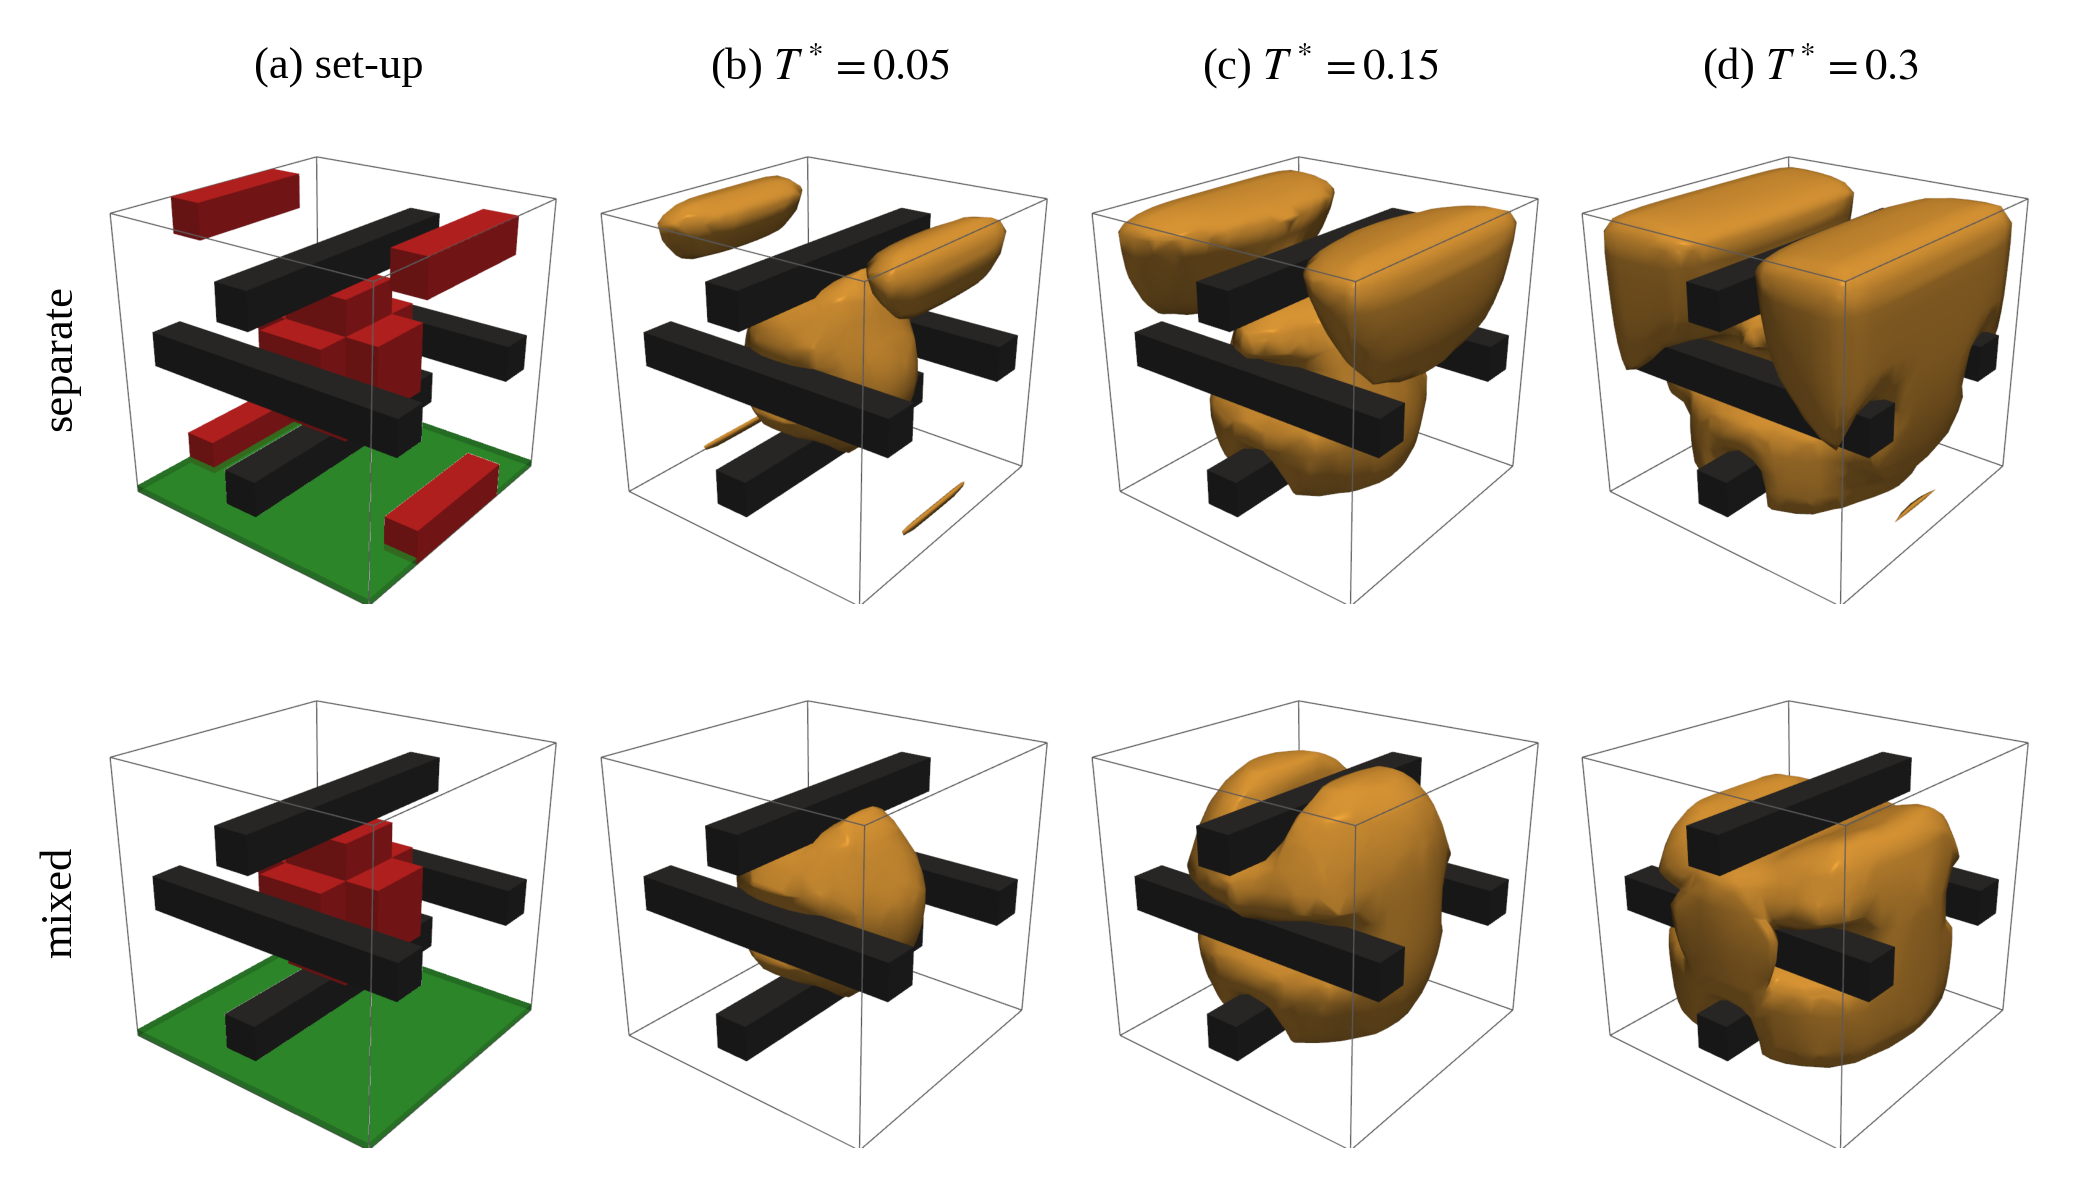
\includegraphics[width=\linewidth]{assets/fig_obstacle_columns_3d.png}
\caption{$\phi_{3D}\ge0.5$ around four rigid bars, separate (top) and mixed (bottom) start; set-up after
Klempt et al.\ (2024), Fig.\ 9.}
\end{figure}
\column{0.34\textwidth}\small
\begin{itemize}\setlength{\itemsep}{6pt}
  \item Four bars after Fig.\ 9 of the paper (positions read off the sketch), no biofilm or nutrient inside,
        frictionless contact
  \item The biofilm grows around the bars and closes behind them, as in Fig.\ 10
  \item The bars restrain the swelling: seed stress about ten times higher than without bars
\end{itemize}
\end{columns}
\end{frame}

% --------------------------------------------------------
\begin{frame}{The maze of Fig.\ 11 with the coupling}
\begin{figure}
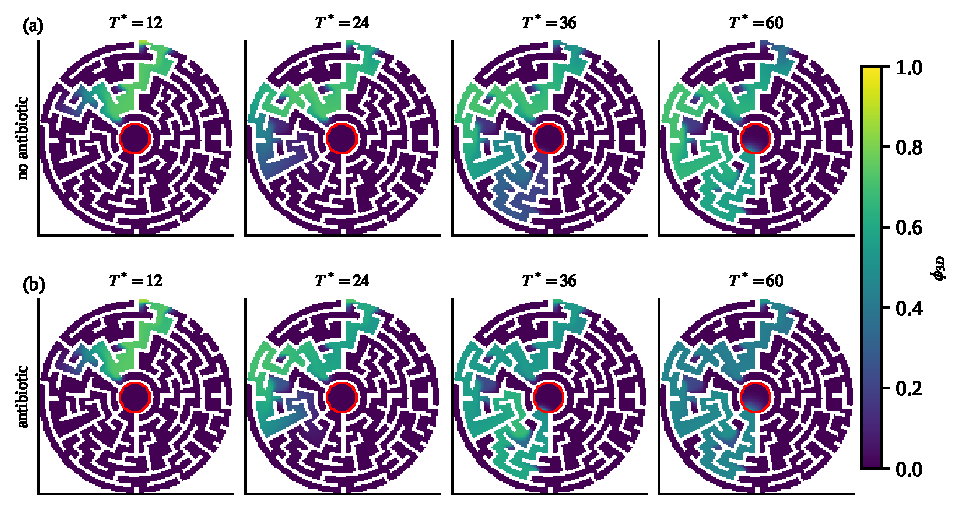
\includegraphics[width=0.66\linewidth]{papers/coupling_paper/fig_maze_k24_h4.pdf}
\caption{$\phi_{3D}$ in the maze of Klempt et al.\ (2024), Fig.\ 11 (560\,\textmu m across, 2D, $h=4$\,\textmu m,
Table 6 constants), without (a) and with (b) antibiotic held at the entrance from $T^*=20$. Nutrient held in the
centre (red), colony at the entrance (top).}
\end{figure}
\vspace{-4pt}\small
The biofilm follows the corridors, also into dead ends, and comes within about 40\,\textmu m of the source by
$T^*=60$; with the antibiotic it stays about 130\,\textmu m away.
\end{frame}

% --------------------------------------------------------
\begin{frame}{Questions and next steps}
\begin{columns}[T]
\column{0.5\textwidth}
\textbf{Questions for you}
\begin{enumerate}\small\setlength{\itemsep}{4pt}
  \item How was the front term stabilised in the runs of Klempt 2024? The cell P\'eclet number is about 25 on the
        paper's mesh.
  \item Can I keep the three element fixes (nearest Gauss point at the surface, conservative Laplacian, neighbours
        by distance)?
  \item Is a stabilised front term acceptable in the thesis, stated as a numerical treatment of Eq.\ 34?
\end{enumerate}
\column{0.46\textwidth}
\textbf{Next steps}
\begin{itemize}\small\setlength{\itemsep}{4pt}
  \item Element runs on $24^3$ with the Lax--Wendroff form for the convergence table
  \item Thesis finished by 4 November with the results up to then
  \item Thesis PDF by 14 December, colloquium on 16 December
  \item A joint paper on the coupling and its verification
\end{itemize}
\end{columns}
\end{frame}

\begin{frame}{References}
\footnotesize
\begin{thebibliography}{9}
\setbeamertemplate{bibliography item}{}
\bibitem{k24} F.~Klempt, M.~Soleimani, P.~Wriggers, P.~Junker. A Hamilton principle-based model for
  diffusion-driven biofilm growth. \emph{Biomech.\ Model.\ Mechanobiol.} 23 (2024) 2091--2113.
\bibitem{k26} F.~Klempt, H.~Geisler, M.~Soleimani, P.~Junker. A continuum multi-species bacterial growth model with a
  novel interaction scheme. \emph{Arch.\ Appl.\ Mech.} 96 (2026) 164.
\bibitem{f25} L.~Fritsch, H.~Geisler, J.~Grashorn, F.~Klempt, M.~Soleimani, M.~Broggi, P.~Junker, M.~Beer. Bayesian
  updating of constitutive parameters under hybrid uncertainties with a novel surrogate model applied to biofilms.
  arXiv:2512.15145 (2025).
\end{thebibliography}
\end{frame}

% ========================================================
\appendix
\begin{frame}{Appendix A: notation}
\small
\begin{tabular}{>{$}l<{$}l}
\toprule
\phi_{3D},\ \alpha & biofilm phase field and growth ($\mathbf F_g=\alpha\mathbf I$, $\alpha(0)=1$), Klempt et al.\ 2024\\
c,\ a & nutrient and antibiotic fields (first and second nutrient field of the element)\\
\beta,\ k_\alpha,\ r,\ k & diffusion of $\phi_{3D}$, growth rate, front speed, Monod constant (Eqs.\ 34, 36)\\
d,\ g & diffusion and uptake of $c$ and $a$ (Eq.\ 35)\\
\phi_i,\ \psi_i,\ \phi_0 & volume fraction and living fraction of species $i$, void (Klempt et al.\ 2026)\\
\bar\phi_i=\phi_i\psi_i & living volume fraction of species $i$; $\sum_i\bar\phi_i$ enters the consumption\\
c^*=c^*_0c,\ \alpha^*=\alpha^*_0a & nutrient and antibiotic seen by the point model (not the growth $\alpha$)\\
T^*,\ s & normalised time; point-model time per unit $T^*$ ($s=0.1$)\\
\bottomrule
\end{tabular}
\end{frame}

\begin{frame}{Appendix B: equations and constants}
\small
\begin{align*}
\dot\phi_{3D}&=\beta\nabla^2\phi_{3D}+k_\alpha\alpha-r\,\tfrac{c}{k+c}\,\mathbf n_c\cdot\nabla\phi_{3D}
  &&\text{(Eq.\ 34 with the front term)}\\
\dot c&=d\nabla^2c-g\,\phi_{3D}\textstyle\sum_i\bar\phi_i\,c,\qquad
\dot a=d\nabla^2a-g\,\phi_{3D}\textstyle\sum_i\bar\phi_i\,a &&\text{(Eq.\ 35; $g\phi$ printed is a misprint)}\\
\dot\alpha&=k_\alpha\,\phi_{3D} &&\text{(Eq.\ 36, unchanged)}
\end{align*}
Point model of Klempt et al.\ 2026 at every Gauss point as published, with $\sum_i\phi_i+\phi_0=1$.

\vspace{2pt}\footnotesize
\begin{tabular}{lll}
\toprule
$\beta$ & 0.02 mm$^2$/$T^*$ & Klempt 2024 Table 2, converted to the 2 mm cube (assumption)\\
$d$, $g$ & $10^8$ mm$^2$/$T^*$, $g\ell^2/d=1$ & Table 2 (fields quasi-steady within $4\times10^{-8}\,T^*$)\\
$r$, $k$, $k_\alpha$ & 10 mm/$T^*$, 1, $10^{-3}$ 1/$T^*$ & Table 2\\
$E$, $\nu$ & 10 Pa, 0.49 & Table 2; void floor $f=10^{-3}$ (converged)\\
point model, $c^*_0$, $s$ & case I, 100, 0.1 & Fritsch et al.\ 2025\\
$\alpha^*_0$, onset & 100 from $T^*=1/3$ & Klempt et al.\ 2026 case 4\\
$\phi_{\min}$ & 0.001 & not in a paper; converged (assumption)\\
\bottomrule
\end{tabular}
\end{frame}

\end{document}
